%!TEX root = ../thesis.tex

\section{経路追従}
経路追従(Path following)とは, 経路計画(Path planning)で引いた経路に対してモビリティが経路を追従できるようにモビリティを制御することである.
基本的にはモビリティのモデルと制御アルゴリズムを利用することで, 最終的にモビリティの入力値(ステアリング角度や並進速度)を計算することが目的となる.

\subsection{PurePursuit}
PurePursuitアルゴリズムは, 経路追従アルゴリズムの中で最も基礎的だが, 非常に広く使われているアルゴリズムである.

PurePursuitはFig.3.1に示すように目標経路上(Path)に対して一定距離先の点を目標点(Look Ahead)とし, その点に到達するようなステアリング制御を行う.
目標点に対してモビリティが前進することで, より先の目標点にたどり着くように制御を行うため, 結果的に目標経路に追従する形となる.

\begin{figure}[H]
  \centering
 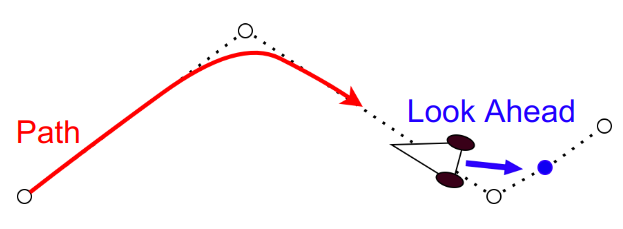
\includegraphics[keepaspectratio, scale=0.5]
      {images/PurePursuit.png}
 \caption{PurePursuit Algorithm}
 \label{fig:purepursuit}
\end{figure}

\section{経路生成}
経路追従を行うためには, 追従するための目標経路(Path)を設定する必要がある.
自律移動モビリティの開発に置いて目標経路の探索を経路計画と呼び, 重要な問題の一つとされている.
本研究では, 目標経路は予め取得した測地座標系の経緯度で用意されたウェイポイントを結ぶ線形経路として設定している.


\subsection{3次スプライン補間}
本研究で取得する目標経路は, ウェイポイントを結ぶ線形経路として設定している.
設定したウェイポイントが疎らである場合に, 離散的で不連続なウェイポイントから, 滑らかで連続的な経路を生成するために3次スプライン補間が使用される.
% そこで, 3次スプライン補間を行うことで, 用意されたウェイポイント上を繋ぐラインに対して曲線を担保することが可能となる.

3次スプライン補間とは, 複数のサンプル点が与えられた時に, そのサンプル点の間を3次の多項式で近似し, 滑らかに保管する手法である.
Fig.3.2にその様子を示す.

\begin{figure}[H]
     \centering
    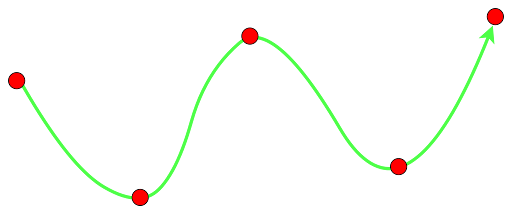
\includegraphics[keepaspectratio, scale=0.5]
         {images/splinepath.png}
    \caption{Spline path}
    \label{fig:purepursuit}
\end{figure}


\newpage